\begin{appendix}
\chapter{Algorithms}
\label{chap:appendix1}

\section{Algorithms detaileds}



\begin{algorithm}

\SetKwInOut{Input}{input}\SetKwInOut{Output}{output}
 \Input{tour $\tau_{1\times n+2}$, state $x_{1 \times n+2}$}
\Output{$\pi$ policy}
$\bar\tau = \tau$\;
$i=1$\;
\While{$x \neq x_f$}{
$\tau = \bar\tau$\;
  \For{$j \in SN$}{
    \If(is the first node in the tour $\tau$, i.e. l=0){i=1}{
      $\tilde{J} = \Gamma(\tau,0,q_l)$\;
      $a_{min} = 0$\;
    }
    \Else{%General case
      $J^0 = g^0(i, \tau_{i+1}, x)$\;
      $J^1 = g^1(i, \tau_{i+1}, x)$\;
      $\tilde{J} = \min\{J^0,J^1\}$\;
      $a = \arg\min\{J^0,J^1\} - 1$\;
    }
    %Evaluate minimization
    \If{$\tilde{J}_{min} > \tilde{J}$}{
      $\tilde{J}_{min} = \tilde{J}$\;
      $a_{min} = a$\;
      $\bar\tau = \tau$\;
      $\tau = sh(\tau,i)$\;
    }
  }
  $l=\bar\tau_{i+1}$\;
  $\pi\leftarrow u=(l,a_{min})$\;
  $x=\Upsilon(x,u)$\;
  \If{$r_l=0$}{
    $SN = SN-l$\;
  }
  $i=i+1$\;
}
\caption{Rollout algorithm}\label{algo:rollout1step}
\end{algorithm}

where SN is the set of nodes that still need to be visited, i.e. $\forall l \in N, D_l > 0$, 
$x_f$ is the final state, where the vehicle comeback to depot and each customer was visited and its demand is $0$, $x=(0,Q,0,\ldots,0)$, $\bar\tau$ is the minimum $\tau$ selected in each algorithm iteration.
$q_l = x_2$, $l=x_1$ and $r_l=x_{l+2}$\\
When $l=0$ or $i=1$ in the algorithm, $q_l = Q$
$sh(\tau,i)$ shift sub $\tau$ vector from position $i$ to the final position. 

The $g^a(l,m,x)$ function is the expected distance from $l$ to $m$ given the state $x$, where $a=1$ if earlier replanishment is specified or $a=0$ in otherwise. The function is described below.
\begin{equation}\label{ra:Cost2Go0}
 g^0(l,m,x)=d(\tau_l,m)+\sum_{k=0}^{q_l}p_m(k)\Gamma(\tau,l+1,q_l-k)+\sum_{k=q_l+1}^{K_m}2d(0,m)p_m(k)\Gamma(\tau,l+1,q_l+Q-k)%Review if \Gamma(\tau,l+1,q_l+Q-k) or \Gamma(\tau,l+1,Q-k)
\end{equation}

\begin{equation}\label{ra:Cost2Go1}
 g^1(l,m,x)=d(0,\tau_l)+d(0,m)+\sum_{k=0}^{K_m}p_m(k)\Gamma(\tau,l+1,Q-k)
\end{equation}


$x_l = \Upsilon(x,u)$ represent the transition of the state $x$ to state $x_l$ given that the control $u$ is realized.


\chapter{Results}

\label{chap:appendix2}

\begin{landscape}

\begin{figure}[!htbp]
  \begin{center}
   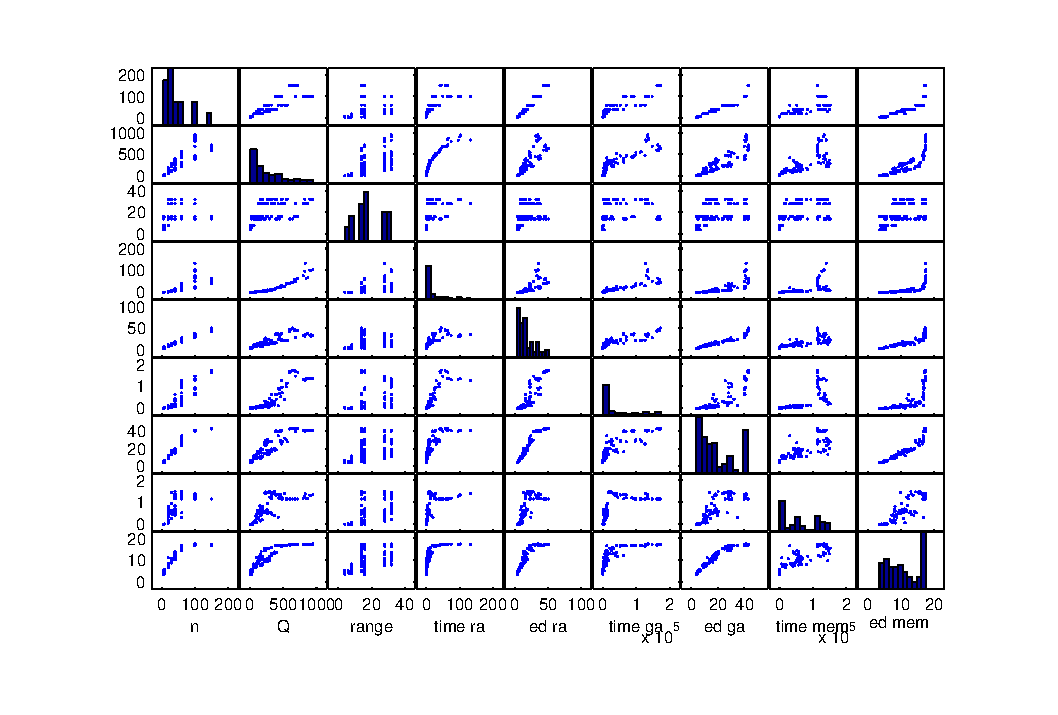
\includegraphics[width=1.4\textwidth]{Images/Chapter5/comparative_results_matrix.eps}
  \end{center}
    \caption{Scatter matrix comparing results and times}\label{fig:comparative_results_matrix}
\end{figure}

\end{landscape}




\subsection{Peformance rollout algorithm}

\begin{figure}[!htbp]
  \begin{center}
   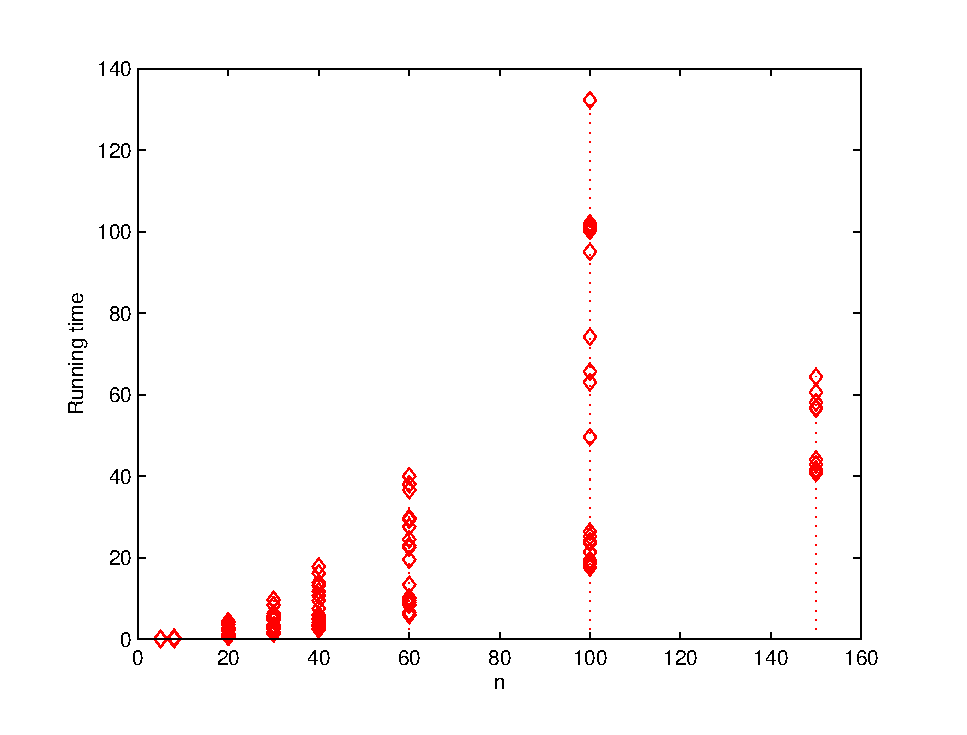
\includegraphics[width=0.9\textwidth]{Images/Chapter5/compare_times_ra.eps}
  \end{center}
    \caption{Time performance evolutionary algorithms}\label{fig:compare_times_ra}
\end{figure}

\begin{figure}[!htbp]
  \begin{center}
   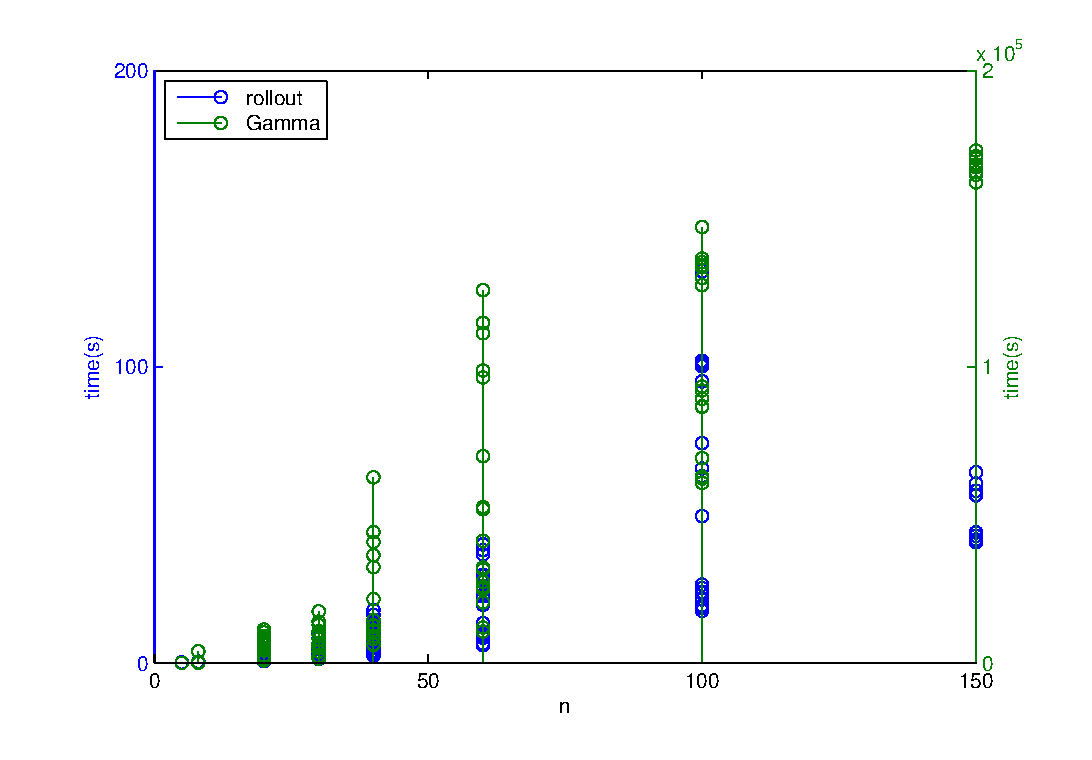
\includegraphics[width=0.9\textwidth]{Images/Chapter5/ra_gamma_time.eps}
  \end{center}
    \caption{Performance rollout algorithm vs. $\Gamma$ algorithm}\label{fig:ra_gamma_time}
\end{figure}

\begin{figure}[!htbp]
  \begin{center}
   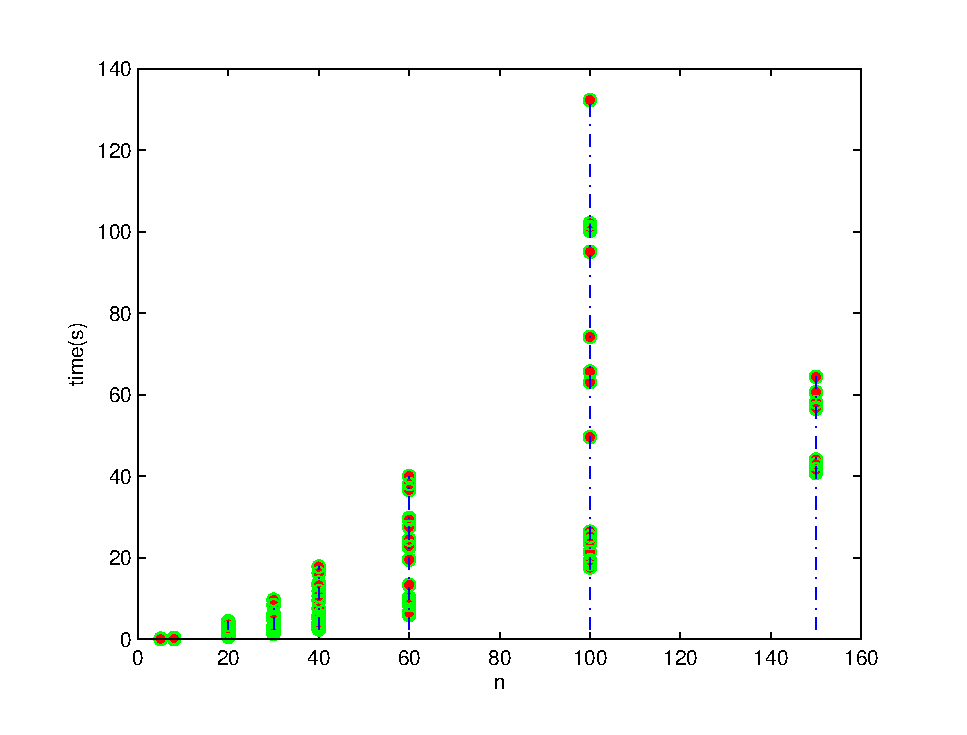
\includegraphics[width=0.9\textwidth]{Images/Chapter5/ra_time.eps}
  \end{center}
    \caption{execution time to accomplish rollout algorithm}\label{fig:expected_distance3D_time}
\end{figure}


\end{appendix}